% Source: StudentGovernmentRepo/Common_Sense_Carolina_Lobbying_org/figures/wing_structure.tex
\documentclass[border=5pt]{standalone}
\usepackage{tikz}
\usepackage{xcolor}
\usetikzlibrary{positioning, arrows.meta, calc, fit, backgrounds}
\definecolor{garnet}{HTML}{73000A}
\definecolor{lightgarnet}{HTML}{F5EAEB}
\definecolor{sandstorm}{HTML}{FFF2E3}
\definecolor{rose}{HTML}{CC2E40}
\definecolor{atlantic}{HTML}{466A9F}
\definecolor{congaree}{HTML}{1F414D}
\definecolor{horseshoe}{HTML}{65780B}
\definecolor{honeycomb}{HTML}{A49137}
\definecolor{grass}{HTML}{CED318}
\definecolor{warmgrey}{HTML}{676156}
\definecolor{tenblack}{HTML}{ECECEC}

\begin{document}
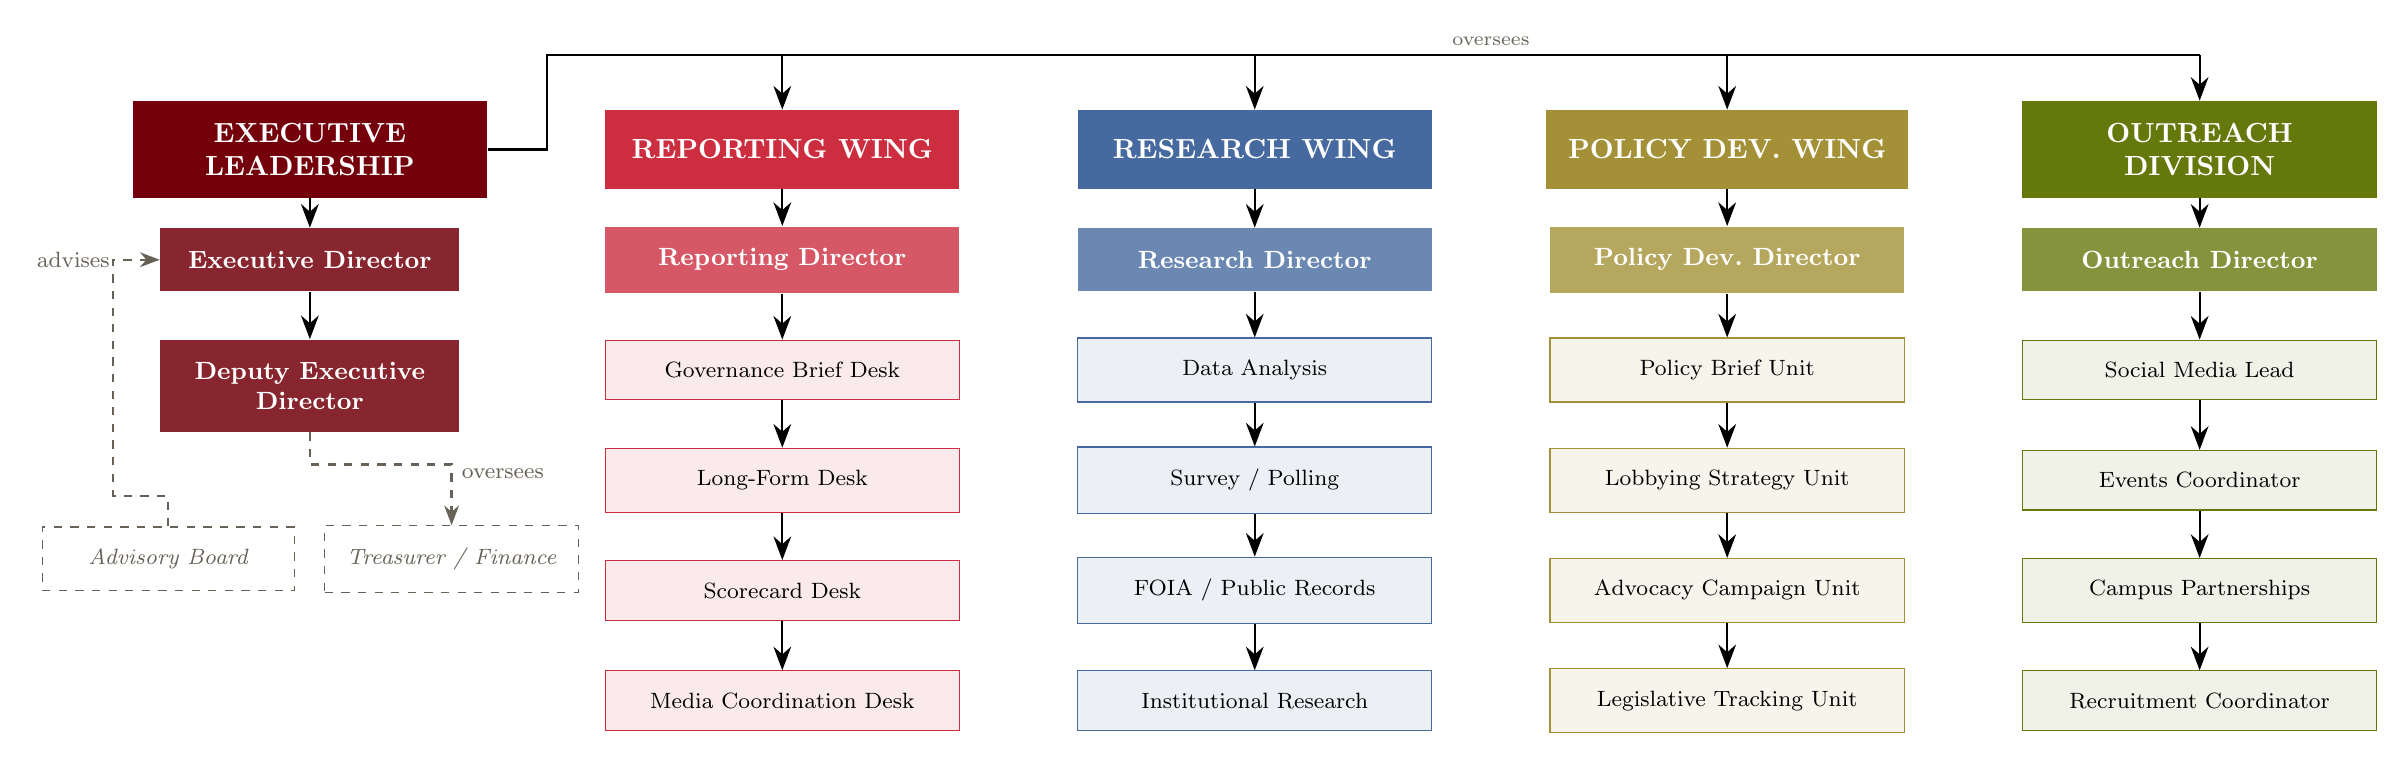
\begin{tikzpicture}[
  every node/.style={sharp corners},
  arr/.style={-{Stealth[length=3mm]}, line width=0.8pt},
  darr/.style={-{Stealth[length=2.5mm]}, line width=0.8pt, dashed, draw=warmgrey},
  hdr/.style={
    rectangle, sharp corners,
    text=white, font=\normalsize\bfseries,
    minimum width=4.5cm, minimum height=1cm,
    align=center, inner sep=8pt
  },
  dirbox/.style={
    rectangle, sharp corners,
    text=white, font=\small\bfseries,
    minimum width=4.5cm, minimum height=0.8cm,
    align=center, inner sep=8pt
  },
  unitbox/.style={
    rectangle, sharp corners,
    text=black, font=\footnotesize,
    minimum width=4.5cm, minimum height=0.7cm,
    align=center, inner sep=8pt
  }
]

%% 5 columns at x=0, 6, 12, 18, 24 (6cm apart)
%% Vertical levels: title=2.5, headers=0, directors=-1.2, units at -2.4, -3.6, -4.8, -6.0

%% ─── COLUMN 1: EXECUTIVE LEADERSHIP (x = 0) ─────────────────────────────────
\node[hdr, fill=garnet] (exec_hdr) at (0, 0)
  {EXECUTIVE\\LEADERSHIP};

\node[dirbox, fill=garnet!85, minimum width=3.8cm] (ed) at (0, -1.4)
  {Executive Director};

\node[dirbox, fill=garnet!85, minimum width=3.8cm] (ded) at (0, -3.0)
  {Deputy Executive\\Director};

\node[unitbox, draw=warmgrey, dashed, fill=none, text=warmgrey,
      font=\footnotesize\itshape, minimum width=3.2cm]
  (advisory) at (-1.8, -5.2) {Advisory Board};

\node[unitbox, draw=warmgrey, dashed, fill=none, text=warmgrey,
      font=\footnotesize\itshape, minimum width=3.2cm]
  (treasurer) at (1.8, -5.2) {Treasurer / Finance};

\draw[arr] (exec_hdr) -- (ed);
\draw[arr] (ed) -- (ded);
%% Advisory Board advises ED (arrow up from board, routed left around deputy)
\draw[darr, -{Stealth[length=2.5mm]}]
  (advisory.north) -- (-1.8, -4.4)
  -- (-2.5, -4.4) -- (-2.5, -1.4)
  -- (ed.west)
  node[pos=0.15, left, font=\footnotesize, text=warmgrey] {advises};
%% Deputy oversees Treasurer (arrow down from deputy, routed right)
\draw[darr]
  (ded.south) -- (0, -4.0)
  -- (1.8, -4.0)
  -- (treasurer.north)
  node[pos=0.15, right, font=\footnotesize, text=warmgrey] {oversees};

%% ─── COLUMN 2: REPORTING WING (x = 6) ───────────────────────────────────────
\node[hdr, fill=rose] (rep_hdr) at (6, 0)
  {REPORTING WING};

\node[dirbox, fill=rose!80] (rep_dir) at (6, -1.4)
  {Reporting Director};

\node[unitbox, fill=rose!10, draw=rose] (rep1) at (6, -2.8)
  {Governance Brief Desk};
\node[unitbox, fill=rose!10, draw=rose] (rep2) at (6, -4.2)
  {Long-Form Desk};
\node[unitbox, fill=rose!10, draw=rose] (rep3) at (6, -5.6)
  {Scorecard Desk};
\node[unitbox, fill=rose!10, draw=rose] (rep4) at (6, -7.0)
  {Media Coordination Desk};

\draw[arr] (rep_hdr) -- (rep_dir);
\draw[arr] (rep_dir) -- (rep1);
\draw[arr] (rep1) -- (rep2);
\draw[arr] (rep2) -- (rep3);
\draw[arr] (rep3) -- (rep4);

%% ─── COLUMN 3: RESEARCH WING (x = 12) ───────────────────────────────────────
\node[hdr, fill=atlantic] (res_hdr) at (12, 0)
  {RESEARCH WING};

\node[dirbox, fill=atlantic!80] (res_dir) at (12, -1.4)
  {Research Director};

\node[unitbox, fill=atlantic!10, draw=atlantic] (res1) at (12, -2.8)
  {Data Analysis};
\node[unitbox, fill=atlantic!10, draw=atlantic] (res2) at (12, -4.2)
  {Survey / Polling};
\node[unitbox, fill=atlantic!10, draw=atlantic] (res3) at (12, -5.6)
  {FOIA / Public Records};
\node[unitbox, fill=atlantic!10, draw=atlantic] (res4) at (12, -7.0)
  {Institutional Research};

\draw[arr] (res_hdr) -- (res_dir);
\draw[arr] (res_dir) -- (res1);
\draw[arr] (res1) -- (res2);
\draw[arr] (res2) -- (res3);
\draw[arr] (res3) -- (res4);

%% ─── COLUMN 4: POLICY DEV. WING (x = 18) ────────────────────────────────────
\node[hdr, fill=honeycomb] (pol_hdr) at (18, 0)
  {POLICY DEV.\ WING};

\node[dirbox, fill=honeycomb!80] (pol_dir) at (18, -1.4)
  {Policy Dev.\ Director};

\node[unitbox, fill=honeycomb!10, draw=honeycomb] (pol1) at (18, -2.8)
  {Policy Brief Unit};
\node[unitbox, fill=honeycomb!10, draw=honeycomb] (pol2) at (18, -4.2)
  {Lobbying Strategy Unit};
\node[unitbox, fill=honeycomb!10, draw=honeycomb] (pol3) at (18, -5.6)
  {Advocacy Campaign Unit};
\node[unitbox, fill=honeycomb!10, draw=honeycomb] (pol4) at (18, -7.0)
  {Legislative Tracking Unit};

\draw[arr] (pol_hdr) -- (pol_dir);
\draw[arr] (pol_dir) -- (pol1);
\draw[arr] (pol1) -- (pol2);
\draw[arr] (pol2) -- (pol3);
\draw[arr] (pol3) -- (pol4);

%% ─── COLUMN 5: OUTREACH DIVISION (x = 24) ───────────────────────────────────
\node[hdr, fill=horseshoe] (out_hdr) at (24, 0)
  {OUTREACH\\DIVISION};

\node[dirbox, fill=horseshoe!80] (out_dir) at (24, -1.4)
  {Outreach Director};

\node[unitbox, fill=horseshoe!10, draw=horseshoe] (out1) at (24, -2.8)
  {Social Media Lead};
\node[unitbox, fill=horseshoe!10, draw=horseshoe] (out2) at (24, -4.2)
  {Events Coordinator};
\node[unitbox, fill=horseshoe!10, draw=horseshoe] (out3) at (24, -5.6)
  {Campus Partnerships};
\node[unitbox, fill=horseshoe!10, draw=horseshoe] (out4) at (24, -7.0)
  {Recruitment Coordinator};

\draw[arr] (out_hdr) -- (out_dir);
\draw[arr] (out_dir) -- (out1);
\draw[arr] (out1) -- (out2);
\draw[arr] (out2) -- (out3);
\draw[arr] (out3) -- (out4);

%% ─── HORIZONTAL CONNECTOR: Executive oversees all wings/divisions ────────────
%% T-junction: ED drops to a horizontal rail, rail spans across all 4 wing headers
\coordinate (rail_left) at (6, 1.2);
\coordinate (rail_right) at (24, 1.2);
\draw[line width=0.8pt] (rail_left) -- (rail_right);

%% ED connects to the rail (plain line, no arrowhead at junction)
\draw[line width=0.8pt] (exec_hdr.east) -- ++(0.75,0) |- (6, 1.2);

%% Vertical drops from rail to each wing header
\draw[arr] (6, 1.2) -- (rep_hdr.north);
\draw[arr] (12, 1.2) -- (res_hdr.north);
\draw[arr] (18, 1.2) -- (pol_hdr.north);
\draw[arr] (24, 1.2) -- (out_hdr.north);

%% Label on the rail
\node[font=\scriptsize, text=warmgrey, above] at (15, 1.2) {oversees};


\end{tikzpicture}
\end{document}
